\chapter{Analyse de l'existant}

L'an passé, un étudiant de la filière FIG, Cédric Patchane, a développé un prototype d'application de Portfolio sur CozyCloud.
Dans cette partie, nous allons faire une analyse de son travail d'un point de vu architecture et de langages utilisés.

\section{Plate-forme de développement utilisée}

\subsection{Présentation de CozyCloud}

CozyCloud est une plateforme de Cloud personnel personnalisable et open-source.  L’outil est entièrement modulaire, et vous offre la possibilité d’installer les fonctionnalités dont vous avez besoin. Il peut s'agir d'applications développées par la communauté ou par vous-même. La différence avec les autres serveurs de Cloud personnel est que Cozy met l'accent sur la collaboration des applications autour des données personnelles de l'utilisateur. Ainsi les applications d'agendas ou de contacts utilisent les mêmes données et sont donc synchronisées. Les applications peuvent être installées depuis la plateforme de développement collaboratif Github ou depuis le catalogue d'application de Cozy ( cf figure 2.2).

\begin{figure}[!ht]
\begin{center}
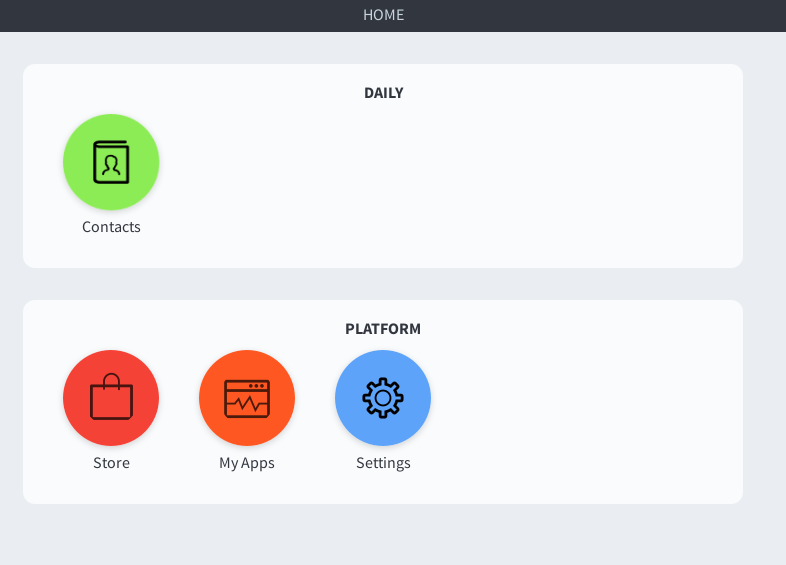
\includegraphics[scale =0.5]{img/cozy_home.png}
\end{center}
\caption{Page home de Cozy Cloud}
\end{figure}

\begin{figure}[!ht]
\begin{center}
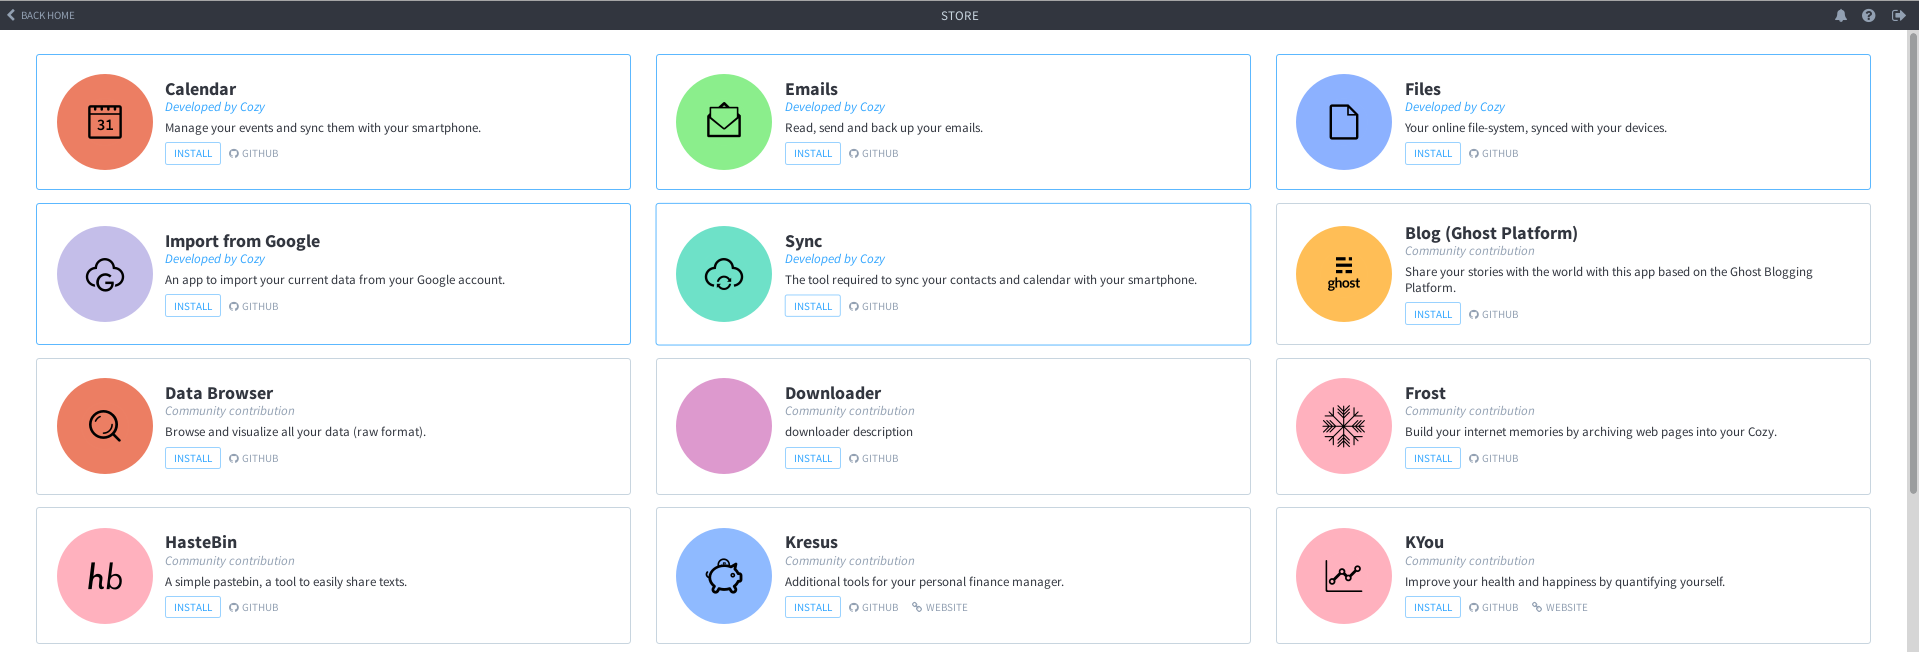
\includegraphics[scale = 0.3]{img/store.png}
\end{center}
\caption{Store de Cozy Cloud}
\end{figure}

\subsection{Architecture et langages utilisés pour le prototype}

Le prototype développé par Cédric Patchane lors de son projet de période 5 se base sur l'architecture de la version 1 de Cozy Cloud. Nous détaillerons ici cette architecture ainsi que le fonctionnement de son application. 

\subsubsection{Environnement de développement}

Pour pouvoir développer des applications pour Cozy, il faut installer un environnement de développement spécifique. En effet, pour pouvoir fonctionner sous CozyCloud, une application nécessite plusieurs outils:\\ 

\textbf{Github :} le premier outil et l'un des plus précieux aux yeux de Cozy est Github. 
Github est un outil de gestion de développement logiciel basé sur le logiciel de version Git. 

Github est l'un des piliers du développement d'applications pour CozyCloud. En effet :

\begin{itemize}
    \item Il favorise la diffusion et le partage de code, et donc de l'open-source.
    \item Mettre son projet sur Github est le seul moyen d'installer une application "maison" sur son Cozy. \\
\end{itemize}

\textbf{Node JS} : Jusqu'à très récemment, le Javascript était uniquement utilisé du côté client. En effet, le navigateur web du visiteur exécutait le Javascript pour effectuer des actions sur la page.
Ceci n'est plus vrai à 100\% désormais. En effet, du code Javascript peut maintenant être exécute du côté serveur. Il est donc désormais possible de générer des pages web directement avec du Javascript. 

Ce serveur NodeJS est donc le second pilier du développement d'applications web pour Cozy cloud. NodeJs permet également de lancer les commandes de développement comme la commande cozy:dev. \\


\textbf{VirtualBox et Vagrant}

VirtualBox est utilisé pour émuler un système d'exploitation complet dans une machine virtuelle. En effet, Cozy est une instance qui tourne sur une machine virtuelle Debian. Celle-ci permet de faire tourner tous les services, comme la base de donnée, etc.

Vagrant est un CLI (Commande Line Interface) qui permet d'interragir avec des commandes avec VirtualBox. Cela permet un développement plus rapide et plus facile. \\

\subsubsection{Présentation de l'architecture de Cozycloud}

La figure~\ref{fig:figArchi} présente la structure de l'architecture de CozyCloud. 

\begin{figure}[!ht]
\begin{center}
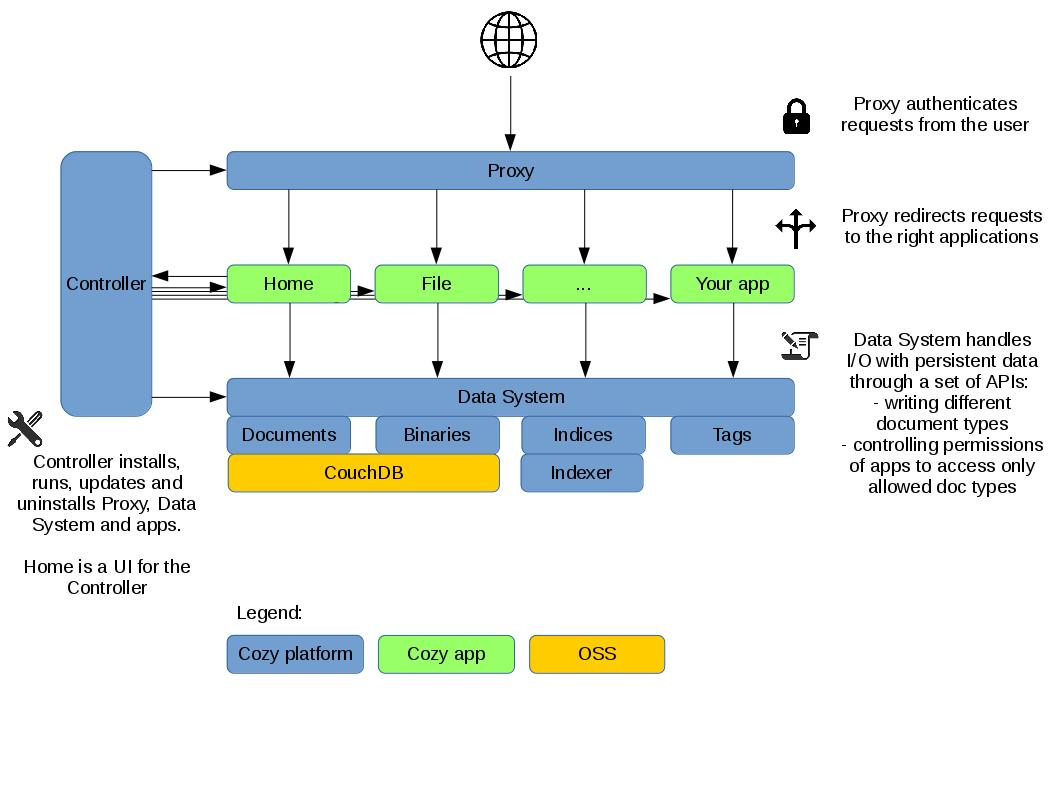
\includegraphics[scale = 0.3]{img/cozy-architecture.jpg}
\end{center}
\caption{Présentation de l'architecture de CozyCloud}
\label{fig:figArchi} 
\end{figure}

\newpage

Cozy est donc constitué de trois composants principaux : \\

\begin{itemize}
    \item La couche data (data-system) : la couche data est au coeur du de l'architecture de cozy. C'est donc la partie centrale où toutes les données sont sécurisées et stockées. La couche data est en fait une API qui consiste à gérer : la database (CouchDB), lieu où sont stockés toutes les données de Cozy. Comme CouchDB est une database de type NOSQL, les données ne sont pas stockées dans des tables, mais sous forme de document (doctypes). Chaques documents sont de types différents et peuvent contenir n'importe quel format de donnée. De plus, avec Cozy, chaque application possède des droits d'accès spécifiques sur ces données, et donc les applications ne sont pas autorisés à accéder à n'importe quelles données de la base. \\

    \item Le Paas (Platform as a service) : c'est l'environnement d'execution des applications. Cela consiste en fait principalement à un contrôleur qui va installer, exécuter, et mettre à jour les applications de Cozy. 
    
    \item L'interface Plateforme : elle consiste en un home et un proxy (répertoire Github). Le home est l'interface qui va permettre au contrôleur de manager les applications dans cozy. Enfin, le proxy va permettre à l'utilisateur d'interagir avec les données. En effet, le proxy va gérer l'authentification et les autorisations d'accès dans Cozy. Ce dernier gère également le "routing", c'est à dire l'envoi de la bonne requête à la bonne application
    
    
\end{itemize}

\subsubsection{Fonctionnalités de l'application}

L'application développées par Cédric permet de réaliser son propre portfolio dans le cloud personnel Cozy. Cette application dispose de quatre vues :

\begin{itemize}
    \item\textbf{Mon profil} : cette vue permet de renseigner les informations du profil utilisateur (nom,prénom...) comme on peut le voir en figure\ref{fig:vueProfil}. L'utilisateur peut choisir d'afficher ou non les informations renseignées sur son portfolio public. 
    \item \textbf{Vue publique du portfolio} : il s'agit de la vue de l'utilisateur générée en fonction des choix d'affichage des documents effectués par l'utilisateur. 
    \item \textbf{Mes choix} : cette vue regroupe tous les documents de l'utilisateur qui peut les modifier ou les supprimer. Il peut également faire le choix de les afficher ou non dans la vue publique de son portfolio. Il est possible d'ajouter des documents directement depuis cette page. 
     \item \textbf{Paramètres} : C'est ici que l'on peut configurer les comptes DoyouBuzz et OpenBadges (cf figure\ref{fig:vueProfil}.    
\end{itemize}

DoYouBuzz est une palteforme de création de CV en ligne. L'application portfolio permet de rapatrier son CV dans son cloud personnel Cozy et ce, via un API. OpenBadges est une représentation de la réussite sous forme de badges. Elle permet de visualiser de façon détaillée l'apprentissage tout au long de la vie d'une personne. Les badges sont récupérés  grâce à l'e-mail associé au compte dans la partie publique d'OpenBadges. Une vue de cette page est disponible en figure~\ref{fig:vueConfigCompte}. 


\begin{figure}[!ht]
\begin{center}
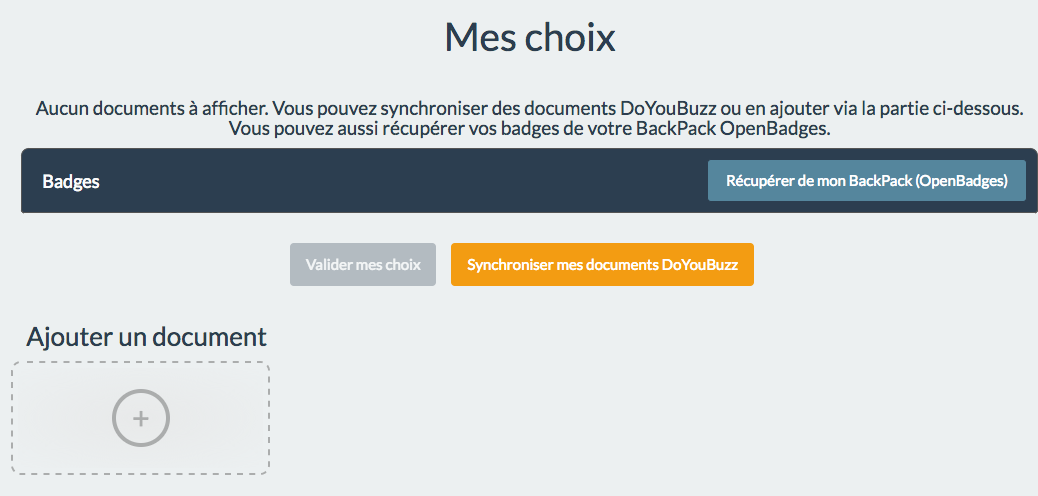
\includegraphics[scale = 0.3]{img/ajout-badges.png}
\end{center}
\caption{Vue de la page ajout des badges}
\label{fig:vueBadge} 
\end{figure}


\begin{figure}[!ht]
\begin{center}
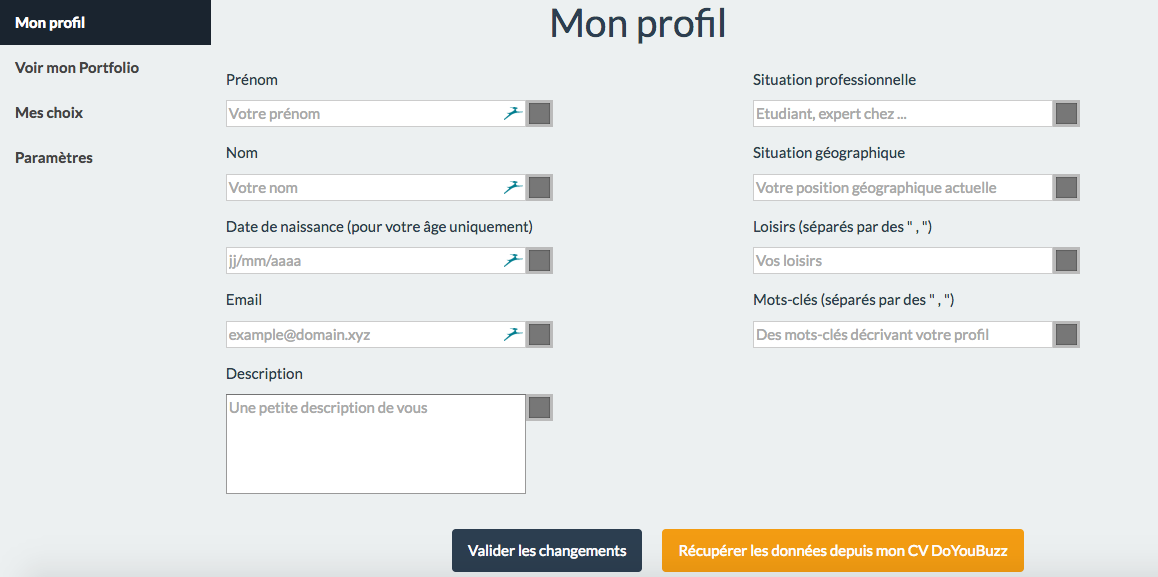
\includegraphics[scale = 0.3]{img/mon-profil.png}
\end{center}
\caption{Vue de la page mon profil}
\label{fig:vueProfil} 
\end{figure}

\begin{figure}[!ht]
\begin{center}
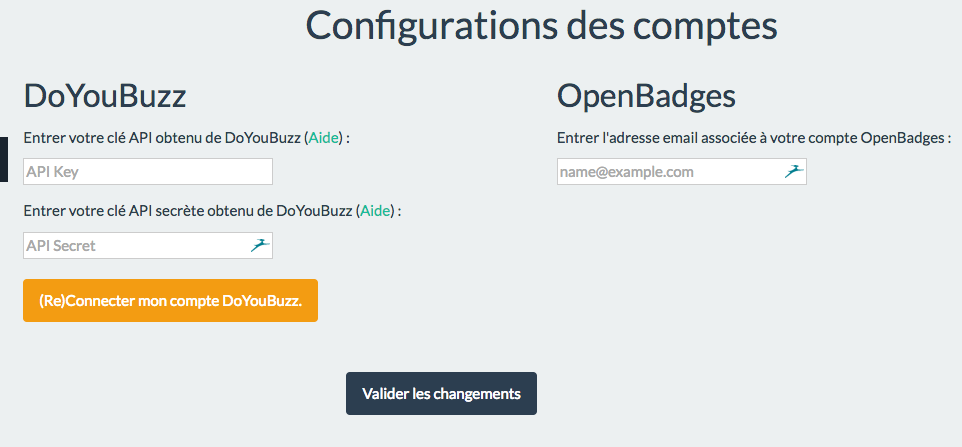
\includegraphics[scale = 0.3]{img/config-comptes.png}
\end{center}
\caption{Vue de la page configuration des comptes}
\label{fig:vueConfigCompte} 
\end{figure}

\section{Choix de repartir d'une nouvelle base}

Après des discussions avec les différents membres présents ou passés du projet (Florian Coste et Cédric Patchane notamment), il nous est apparu nécessaire de repartir sur une nouvelle base. En effet, l'architecture de Cozy est en pleine évolution et la v3 devrait être disponible dans les prochains mois (annoncée pour mars 2017). L'application développée par Cédric correspond à une architecture type v1 et est décomposée en une partie cliente et une partie serveur. Cette dernière est difficilement maintenable par le développeur d'applications au gré des évolutions de librairies tierces par exemple. Le choix de l'équipe de Cozy fut de pousser le développement d'applications de type "clientsideapps" ou la partie serveur n'est plus gérée par le développeur mais par Cozy. Nous avons fait le choix de développé de cette manière pour rendre compatible notre application avec la version 2. A terme, nous nous sommes assurés par le biais d'échanges avec l'équipe Cozy (Cédric mais aussi le channel IRC), que l'application serait facilement migrable vers la version 3. 

Pour conclure cette partie, on peut donc dire que la phase d'analyse nous a permis de comprendre l'existant mais aussi de se rendre compte qu'il fallait en modifier l'architecture. Nous verrons plus en détail par la suite, les choix que nous avons effectués. 


